% Options for packages loaded elsewhere
\PassOptionsToPackage{unicode}{hyperref}
\PassOptionsToPackage{hyphens}{url}
\PassOptionsToPackage{dvipsnames,svgnames,x11names}{xcolor}
%
\documentclass[
  letterpaper,
  DIV=11,
  numbers=noendperiod]{scrartcl}

\usepackage{amsmath,amssymb}
\usepackage{lmodern}
\usepackage{iftex}
\ifPDFTeX
  \usepackage[T1]{fontenc}
  \usepackage[utf8]{inputenc}
  \usepackage{textcomp} % provide euro and other symbols
\else % if luatex or xetex
  \usepackage{unicode-math}
  \defaultfontfeatures{Scale=MatchLowercase}
  \defaultfontfeatures[\rmfamily]{Ligatures=TeX,Scale=1}
\fi
% Use upquote if available, for straight quotes in verbatim environments
\IfFileExists{upquote.sty}{\usepackage{upquote}}{}
\IfFileExists{microtype.sty}{% use microtype if available
  \usepackage[]{microtype}
  \UseMicrotypeSet[protrusion]{basicmath} % disable protrusion for tt fonts
}{}
\makeatletter
\@ifundefined{KOMAClassName}{% if non-KOMA class
  \IfFileExists{parskip.sty}{%
    \usepackage{parskip}
  }{% else
    \setlength{\parindent}{0pt}
    \setlength{\parskip}{6pt plus 2pt minus 1pt}}
}{% if KOMA class
  \KOMAoptions{parskip=half}}
\makeatother
\usepackage{xcolor}
\setlength{\emergencystretch}{3em} % prevent overfull lines
\setcounter{secnumdepth}{-\maxdimen} % remove section numbering
% Make \paragraph and \subparagraph free-standing
\ifx\paragraph\undefined\else
  \let\oldparagraph\paragraph
  \renewcommand{\paragraph}[1]{\oldparagraph{#1}\mbox{}}
\fi
\ifx\subparagraph\undefined\else
  \let\oldsubparagraph\subparagraph
  \renewcommand{\subparagraph}[1]{\oldsubparagraph{#1}\mbox{}}
\fi


\providecommand{\tightlist}{%
  \setlength{\itemsep}{0pt}\setlength{\parskip}{0pt}}\usepackage{longtable,booktabs,array}
\usepackage{calc} % for calculating minipage widths
% Correct order of tables after \paragraph or \subparagraph
\usepackage{etoolbox}
\makeatletter
\patchcmd\longtable{\par}{\if@noskipsec\mbox{}\fi\par}{}{}
\makeatother
% Allow footnotes in longtable head/foot
\IfFileExists{footnotehyper.sty}{\usepackage{footnotehyper}}{\usepackage{footnote}}
\makesavenoteenv{longtable}
\usepackage{graphicx}
\makeatletter
\def\maxwidth{\ifdim\Gin@nat@width>\linewidth\linewidth\else\Gin@nat@width\fi}
\def\maxheight{\ifdim\Gin@nat@height>\textheight\textheight\else\Gin@nat@height\fi}
\makeatother
% Scale images if necessary, so that they will not overflow the page
% margins by default, and it is still possible to overwrite the defaults
% using explicit options in \includegraphics[width, height, ...]{}
\setkeys{Gin}{width=\maxwidth,height=\maxheight,keepaspectratio}
% Set default figure placement to htbp
\makeatletter
\def\fps@figure{htbp}
\makeatother

\KOMAoption{captions}{tableheading}
\makeatletter
\makeatother
\makeatletter
\makeatother
\makeatletter
\@ifpackageloaded{caption}{}{\usepackage{caption}}
\AtBeginDocument{%
\ifdefined\contentsname
  \renewcommand*\contentsname{Table of contents}
\else
  \newcommand\contentsname{Table of contents}
\fi
\ifdefined\listfigurename
  \renewcommand*\listfigurename{List of Figures}
\else
  \newcommand\listfigurename{List of Figures}
\fi
\ifdefined\listtablename
  \renewcommand*\listtablename{List of Tables}
\else
  \newcommand\listtablename{List of Tables}
\fi
\ifdefined\figurename
  \renewcommand*\figurename{Figure}
\else
  \newcommand\figurename{Figure}
\fi
\ifdefined\tablename
  \renewcommand*\tablename{Table}
\else
  \newcommand\tablename{Table}
\fi
}
\@ifpackageloaded{float}{}{\usepackage{float}}
\floatstyle{ruled}
\@ifundefined{c@chapter}{\newfloat{codelisting}{h}{lop}}{\newfloat{codelisting}{h}{lop}[chapter]}
\floatname{codelisting}{Listing}
\newcommand*\listoflistings{\listof{codelisting}{List of Listings}}
\makeatother
\makeatletter
\@ifpackageloaded{caption}{}{\usepackage{caption}}
\@ifpackageloaded{subcaption}{}{\usepackage{subcaption}}
\makeatother
\makeatletter
\@ifpackageloaded{tcolorbox}{}{\usepackage[many]{tcolorbox}}
\makeatother
\makeatletter
\@ifundefined{shadecolor}{\definecolor{shadecolor}{rgb}{.97, .97, .97}}
\makeatother
\makeatletter
\makeatother
\ifLuaTeX
  \usepackage{selnolig}  % disable illegal ligatures
\fi
\IfFileExists{bookmark.sty}{\usepackage{bookmark}}{\usepackage{hyperref}}
\IfFileExists{xurl.sty}{\usepackage{xurl}}{} % add URL line breaks if available
\urlstyle{same} % disable monospaced font for URLs
\hypersetup{
  pdftitle={Mappeoppgave2},
  pdfauthor={31 \& 39},
  colorlinks=true,
  linkcolor={blue},
  filecolor={Maroon},
  citecolor={Blue},
  urlcolor={Blue},
  pdfcreator={LaTeX via pandoc}}

\title{Mappeoppgave2}
\author{31 \& 39}
\date{}

\begin{document}
\maketitle
\ifdefined\Shaded\renewenvironment{Shaded}{\begin{tcolorbox}[sharp corners, borderline west={3pt}{0pt}{shadecolor}, interior hidden, frame hidden, boxrule=0pt, breakable, enhanced]}{\end{tcolorbox}}\fi

Modellen som brukes i oppgaven:

\[
𝑦− 𝑦_𝑛 = 𝑧 − 𝛼(𝑖 − 𝜋_𝑒)
\]

\[
𝑖 = 𝜙_𝑦(𝑦 − 𝑦_𝑛) + 𝜙_𝜋(𝜋 − 𝜋^∗)
\]

\[ 
𝜋 = 𝜋_𝑒 + 𝛽(𝑦 − 𝑦_𝑛) 
\]

Her er 𝑦, 𝑖 og 𝜋 henholdsvis produksjon, nominell rente, og prisvekst.

\textbf{Oppgave 1a: IS-RR-PK}

Parameteren 𝛼 avhenger av hvordan økonomien fungerer. Da med hensyn til
hvor følsom \(y\) er til faktorer som investering og konsum i en lukket
økonomi.

\[
𝛼 = \frac{𝛥y}{𝛥i}
\]

Her vil 𝛼 representere følsomheten til produksjonsgapet med hensyn til
endringer i den nominelle renten Δ𝑖. Dersom den nominelle renten øker,
vil produksjonsgapet endre seg med 𝛼 for hvert prosentpoeng av den
nominelle renten.

Hvis vi antar at produksjonsgapet avhenger av investeringer og konsum.
Kan vi skrive produksjonsgapet som en funksjon av disse:

\[
Δ𝑦 = f(Investering, Konsum) 
\]Investeringene påvirkes av den nominelle renten. Dermed kan vi
derivere Δ𝑦 med hensyn til Δ𝑖 og finne den tilsvarende følsomheten :

\[
𝛼 = \frac{Δ𝑦}{Δ𝑖} = \frac{∂Δ𝑦}{∂investering}\frac{∂Investering}{∂Δ𝑖}
\]

Dermed blir 𝛼 følsomheten til produksjonsgapet med hensyn til
investeringer, og følsomheten til investeringene med hensyn til den
nominelle renten. Visst vi antar at investeringer er følsomme for
endringer i nominelle rente vil parameteren være høy. Dersom det blir
dyrere å låne penger, og man er avhengig av å ta opp lån, vil det dermed
bli vanskelig selv med små endringer i den nominelle renten. Videre vil
en reduksjon i investeringer påvirke BNP og produksjonsgapet.

Derfor vil verdien på parameteren 𝛼 avhenge av hvordan økonomien
fungerer, spesielt hvor følsomme investeringene er for endringer i den
nominelle renten.

\textbf{Oppgave 1b}

Vi bruker ligningene i den enkle modellen til å løse for \(y\) der
\(y_n = 0\) . Starter med å sette 3 inn i 2 og løser deretter for y:

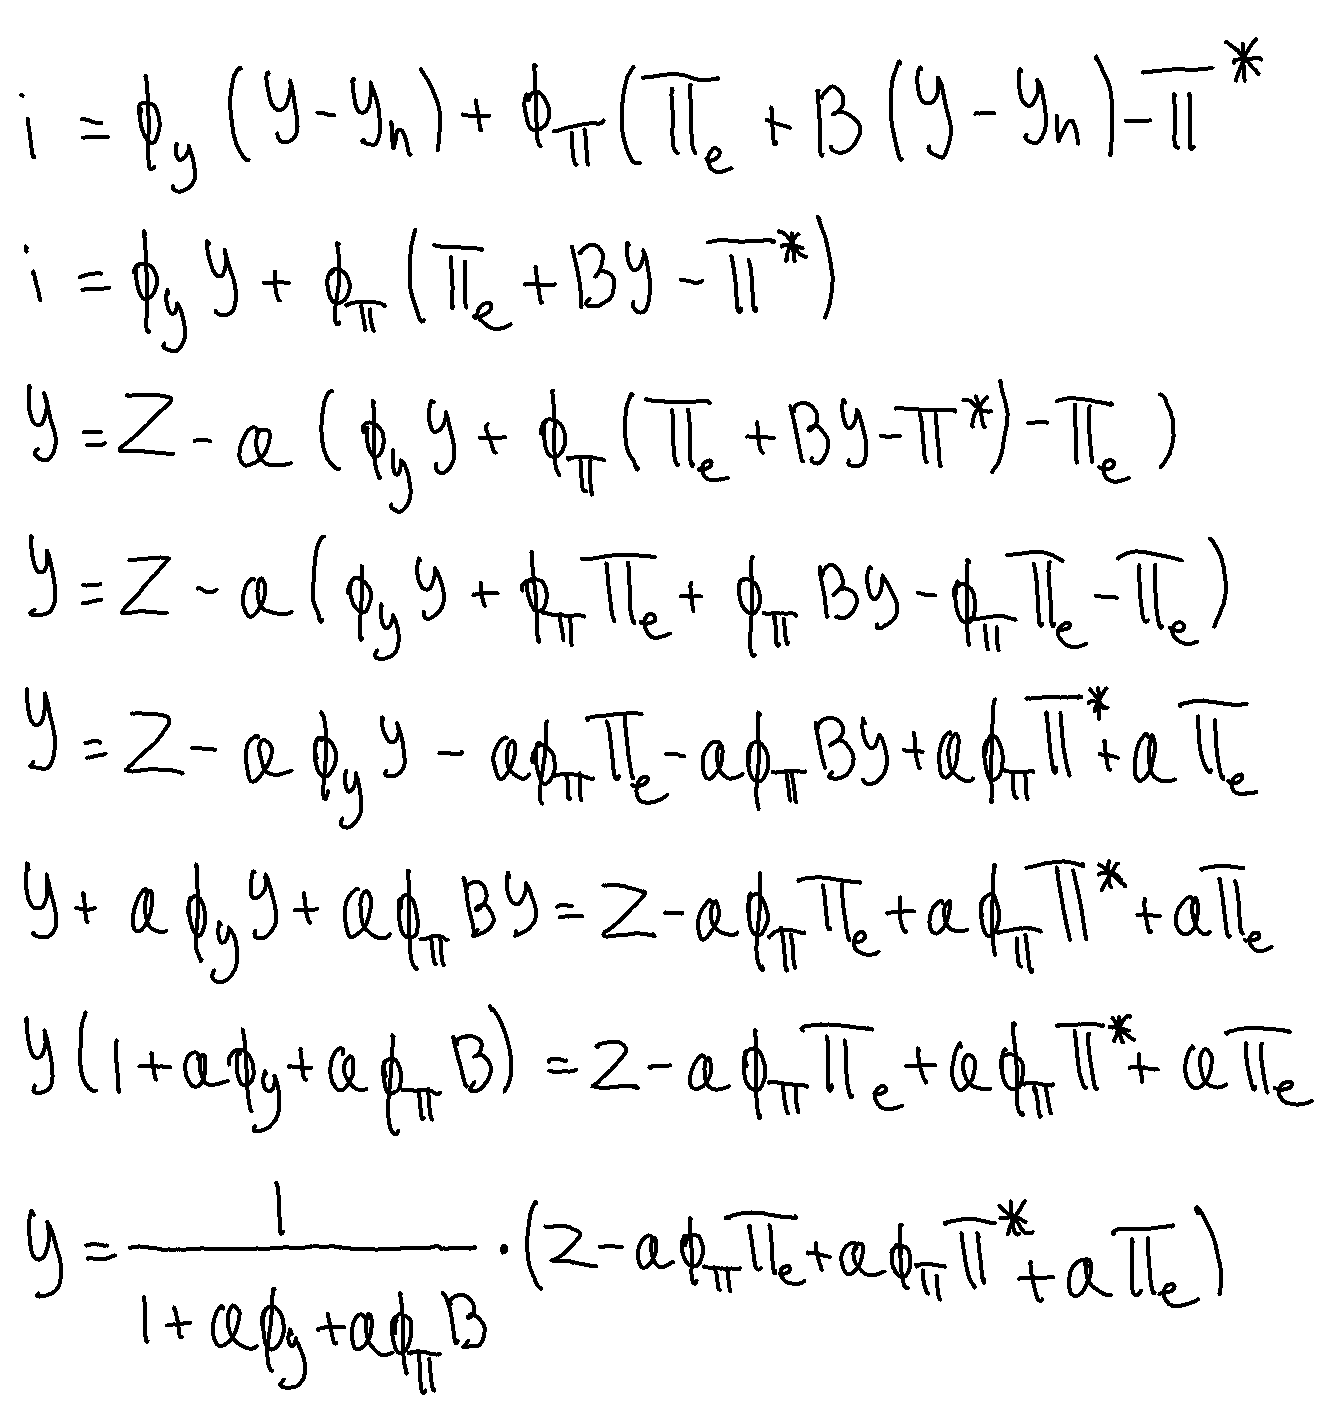
\includegraphics[width=5.17708in,height=\textheight]{images/Quick sheets - page 3.png}

En økning i forventet inflasjon innebærer lavere realrente (prisen på
penger går ned), og dermed øker etterspørselen i økonomien, noe som
igjen fører til inflasjon. For å motvirke inflasjonen setter
sentralbanken opp styringsrenten. Renteesettingen avhenger av \(y\) og
de eksogene variablene:

\[
𝑖 = 𝜙_𝑦(𝑦 − 𝑦_𝑛) + 𝜙_𝜋(𝜋_𝑒 + 𝛽(𝑦 − 𝑦_𝑛) − 𝜋^∗) 
\]

RR - kurven skifter opp og endringen i nominell rente blir positiv:

\[
𝛥i = 𝜙_𝜋𝛥𝜋_𝑒 > 0
\]

Økningen i forventet inflasjon fører til økt lønns- og prisvekst. PK -
kurven skifter opp og endringen i prisveksten er positiv:

\[ 𝛥𝜋 = 𝛥𝜋^e > 0 \]

Produksjonen faller kun hvis \(𝜙_𝜋 > 1\). Av ligning 2 ser vi at visst
inflasjonen \(𝜋\) ligger på sin målverdi på 2\% og vi setter
koeffisienten som et tall under 1 (har brukt 0,5 som et eksempel), så
vil ikke den nominelle renten øke mer enn inflasjonen, noe som fører til
realrenten ikke økes, og at produksjon dermed ikke faller. Koeffisienten
må derfor være større enn 1 for at realrenten skal kunne bekjempe
inflasjonen.

\[ 𝑖 = 𝜙_𝑦(𝑦 − 𝑦_𝑛) + 0,5(𝜋 − 0,02) \]

\textbf{Oppgave 2: Adaptive forventninger}

Ligning for adaptive inflasjonsforventninger:

\[
𝜋_t = 𝜋_𝑡^e + 𝛽(𝑦_𝑡 − 𝑦_𝑛)
\]

Antar adaptive forventninger ved:

\[
𝜋_t^e = 𝜋_𝑡−1
\]

Når produksjonsgapet holdes positivt (summen av parentesen blir
positiv), altså større en nivået for potensielt BNP, vil inflasjon øke.
Når det er adaptive forventninger vil inflasjons- forventningene
oppdateres i neste periode, og siden produksjonsgapet er positivt vil
PK-kurven forflytte seg oppover. Inflasjonen blir altså høyere enn
aktørene forventer, og ved neste periode vil aktørene forvente høyere
inflasjon. Kurven vil dermed forsette å forflytte seg oppover så lenge
produksjon er over det potensielle nivået, og således vil prisveksten
stige mer og mer. Dette er illustrert i figuren under der
\(𝜋^0\),\(𝜋^1\) og \(𝜋^2\) er nivåer på inflasjon. Det naturlige nivået
på produksjon vises som \(y_n\) , mens \(y_t\) er nivået på produksjon
som den ekspansive økonomiske politikken forsøker å holde.

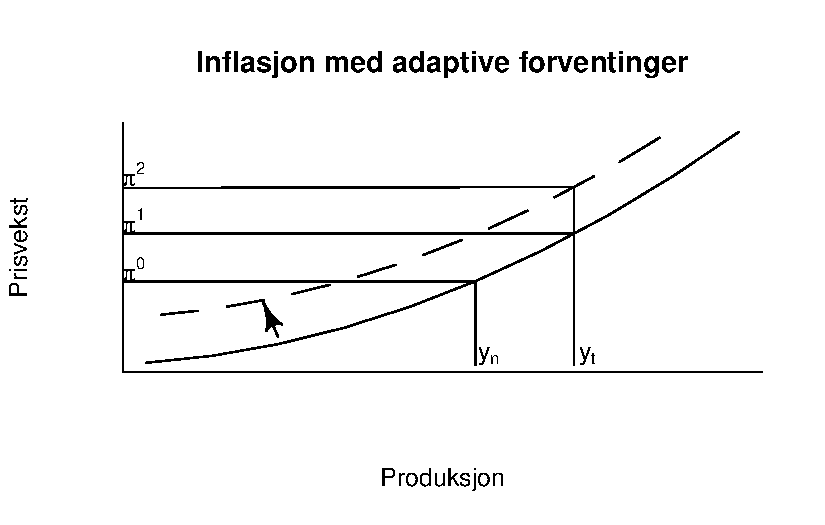
\includegraphics{31_SOK1016_M2_V23.pdf._files/figure-pdf/unnamed-chunk-2-1.pdf}

Dette er ikke en rimelig antagelse over tid, fordi det på sikt fører til
hyperinflasjon. Det kan ikke være langsiktig likevekt med adaptive
forventninger, på grunn av at inflasjonen blir større enn forventet
inflasjon. Vi trenger derfor mekanismer som bringer produksjon
(ledigheten) tilbake til det naturlige nivået.

\textbf{Oppgave 3}

Norges bank har i dag et inflasjonsmål om en prisvekst på 2 prosent for
hvert år. Dette er for å kunne oppnå en stabil og bærekraftig vekst i
det norske markedet. Norge har klart seg forholdsvis greit med å holde
seg på dette inflasjonsmålet. Men etter en pandemi som forstyrret
økonomien, har det gitt en prisstigning som har blitt et stadig et
større problem.

Prisveksten var relativ lav under pandemien i 2020 og inn mot 2021.
Norge hadde i en lang periode ekspansiv pengepolitikk, med lav
styringsrente fra Norges bank. I ettertiden brukte mange i befolkningen
mye penger, som ble oppspart under lockdown. Dette resulterte i en høy
prisvekst.

Som en konsekvens av den økende prisveksten, har mange nordmenn opplevd
en lavere kjøpekraft og reallønn. Mat, strøm og andre nødvendighetsgoder
har økt mye. Dette har påvirket nordmenns kjøpemønstre, spesielt for
innbyggere med lav inntekt. Luksusvarer, reise og andre goder med høy
priselastisitet er eksempler på goder som har opplevde en synkende
etterspørsel. Den lave kjøpekraften blir heller ikke hjulpet av
pengepolitikken som innføres av Norges bank. I et forsøk på å senke
prisveksten har styringsrenten blitt gradvis hevet siden den historiske
nullrenten.

Økte priser på råvarer og transport har bidratt til økte kostnader for
bedrifter. Samtidig opplever de lavere etterspørsel for sine produkter,
siden konsumentene opplever en lavere kjøpekraft. Senere
lønnsforhandlinger gjør at prisen for arbeidskraft stiger ytterligere.

I en undersøkelse gjennomført av Ipsos, spør de ulike grupper om den
forventede prisveksten. Blant disse gruppene er økonomieksperter og
husholdninger. Her forventet økonomene en prisvekst på 4,3 prosent de
neste 12 månedene. Dette var 0,6 prosentpoeng lavere enn forrige
kvartal. For husholdningene derimot var det forventet en økning på 6
prosent de neste 12 månedene. Her er det en økning på 1,9 prosentpoeng
siden forrige kvartal (Ludvigsen, 2023). Dette viser at det er delte
meninger om hvordan den fremtidige prisveksten vil utvikle seg.

\textbf{Kildeliste}:

Ludvigsen, (2023). Forventningsundersøkelsen. Norges Bank. Hentet fra:
\href{https://www.norges-bank.no/contentassets/7905f518185c4d8d8cf91bc3c340cdde/forventningsundersokelsen-for-norges-bank-1.-kvartal-2023.pdf?v=02\%2F16\%2F2023185104\&ft=.pdf\&fbclid=IwAR1XIlF3_PgeJVznmS9dRjSK8gqkRlow4pYafmM8VhM7mLsFYRYC5D0qs0I}{https://www.norges-bank.no/contentassets/7905f518185c4d8d8cf91bc3c340cdde/forventningsundersokelsen-for-norges-bank-1.-kvartal-2023.pdf?v=02/16/2023185104\&ft=.pdf}



\end{document}
